\section{Symbolic Regression: Stochastic}
\label{sr_stochastic}
With the extended symbolic regression implementation, we move on to the stochastic approach. In this approach, we introduce the concept of \emph{stochastic node}, which is a versatile node that integrates the functions \textbf{add}, \textbf{sub}. \textbf{mul} and \textbf{div} in it. An probability is associated to each of the functions so that when a stochastic node is evaluated, the function of the node is determined (randomly) by their probabilities. 

\subsection{Representation}
In our approach, there is only one function node: \textbf{OPNode}. There are two terminal nodes \textbf{X} and \textbf{Y}. In order to model the probability mechanism, we introduce four additional terminals: \textbf{One} (1), \textbf{Two} (2), \textbf{Three} (3) and \textbf{Four} (4). Instead of giving these nodes the \emph{nil} type (ECJ's default type), we give these nodes the \emph{int} type, so that they can be distinguished from the nodes of \emph{nil} type in the tree. %The \emph{OPNode} has ten children of type \emph{int}, when an \emph{OPNode} is evaluated, it evaluates the ten children to determine the probabilities of the functions.
\begin{figure}
	\centering
	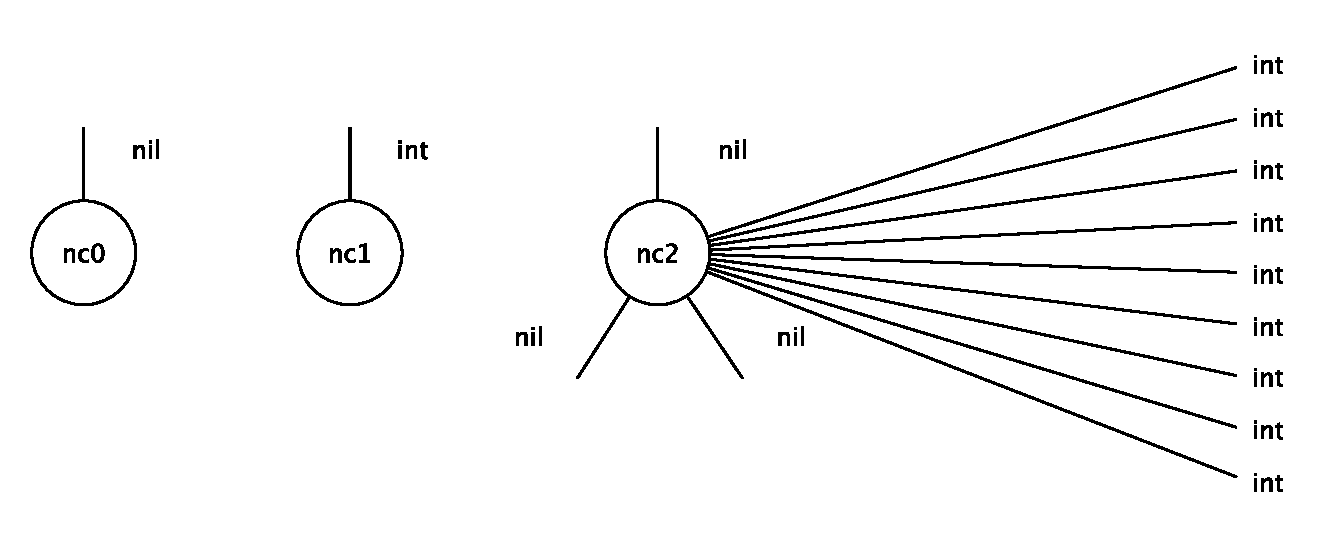
\includegraphics[width=1\linewidth]{./fig/symbolic_stochastic_ncs}
	\caption{Node constraints for the symbolic regression problem.}
	\label{fig:symb_stochastic_ncs}
\end{figure}

To implement the stochastic node we define the node constraints shown in Figure \ref{fig:symb_stochastic_ncs}. \emph{nc0} is unchanged as it is used for terminals \textbf{X} and \textbf{Y}. \emph{nc1} specifies that the nodes which conform to it should have no children and their return types as \emph{int}. In our approach, nodes \textbf{One}, \textbf{Two}, \textbf{Three} and \textbf{Four} conform to \emph{nc1}. \emph{nc2} specifies that the nodes which conform to it should have 2 nodes of type \emph{nil}, 10 nodes of type \emph{int} and its own return type as \emph{nil}. In our approach, the function nodel \textbf{OPNode} conforms to \emph{nc2}. 



\subsection{Function weightings and stochastic costs}
The probability and the selection of the function of an \emph{OPNode} is explained as follows;

\begin{itemize}
	\item Each \emph{OPNode} keeps track of the \emph{weight}s of functions \textbf{add}, \textbf{sub}, \textbf{mul} and \textbf{div}, denoted by $W_{add}$, $W_{sub}$, $W_{mul}$ and $W_{div}$. Initially they are all 0.
	\item When an \emph{OPnode} is evaluated, the ten nodes of type \emph{int} are evaluated first. When node \textbf{One} is encountered, $W_{add}$ is increased by 1. $W_{sub}$, $W_{mul}$ and $W_{div}$ are increased by 1 if nodes \textbf{Two}, \textbf{Three} and \textbf{Four} are encountered respectively.
	\item The probability of the functions are calculated based on their weights. In particular, let $P_{add}$, $P_{sub}$, $P_{mul}$ and $P_{div}$ denote the probabilities of \textbf{add}, \textbf{sub}, \textbf{mul} and \textbf{div}. Such that
	\begin{align*}
	P_{add} = W_{add} / (W_{add} + W_{sub} + W_{mul} + W_{div})\\
	P_{sub} = W_{sub} / (W_{add} + W_{sub} + W_{mul} + W_{div})\\
	P_{mul} = W_{mul} / (W_{add} + W_{sub} + W_{mul} + W_{div})\\
	P_{div} = W_{div} / (W_{add} + W_{sub} + W_{mul} + W_{div})
	\end{align*}
	\item The function of the \emph{OPNode} is then selected randomly by the probabilities $P_{add}$, $P_{sub}$, $P_{mul}$ and $P_{div}$.
	\item Each \emph{OPNode} is also associated with a \emph{stochastic cost}, denoted by $N_{stochastic}$, such that:
	\begin{align*}
	N_{stochastic} = 1 - max(P_{add}, P_{sub}, P_{mul}, P_{div})
	\end{align*}
	to calculate the stochastic cost of a tree ($T_{stochastic}$), in our approach, we use the sum of the \emph{stochastic cost}s of all the \emph{OPNode}s in a tree:
	\begin{align*}
	T_{stochastic} = \sum\nolimits_{N \in OPNodes} N_{stochastic}
	\end{align*}
\end{itemize}

\subsection{Fitness}
The objective of the stochastic symbolic regression is the same as the symbolic regression. In our approach we use the same experiment settings (same upfront equations, 20 randomised values for each \textbf{X} and \textbf{Y}, and their expected results $ev$). In addition, we add another search objective: to minimise the \emph{stochastic cost} ($T_{stochastic}$) of the tree. Let $v$ denote the value retured by evaluating a tree, we define our secondary fitness:
\begin{align}
fitness = abs(ev - v) + T_{stochastic} \label{eq:1}
\end{align}

During the evolutionary process, for each pair of \textbf{X} and \textbf{Y}, the tree is evaluated 100 times and the lowest fitness cost is kept.

Through experimentation, we observe that the weightings of the objectives are significant to the evolutionary process. We observe that if the two objectives share the same weighting (as in Equation \ref{eq:1}), the stochastic cost dominates the evolution, causing the main tree (the tree containing \emph{OPNode}s only, not the subtrees of each \emph{OPNode}) to stop evolving from early generations. We then search for the weightings of the two objectives and observe that the factor of 0.01 should be applied to the stochastic cost in order to balance the two objectives. Thus, we refine our fitness:

\begin{align}
fitness = abs(ev - v) + 0.01*T_{stochastic} \label{eq:2}
\end{align}

With the refined fitness, we observe that the global optimal is obtained within 80 generations of evolution. The stochastic cost of the final tree is zero as a result of evolution, this means that each node in the tree is deterministic, i.e. it only has one function every time it is evaluated. 

